\documentclass{article}
\usepackage{amsmath}
\usepackage{amssymb}
\usepackage[a4paper, top=25mm, bottom=25mm, left=25mm, right=25mm]{geometry}
\usepackage{pgfplots}
\pgfplotsset{compat=1.18}
\usepackage{mathtools}
\usepgfplotslibrary{polar}
\usepgfplotslibrary{fillbetween}

\begin{document}
\pagestyle{empty}
\large

\begin{center}
2023-2024 Fall \\MAT124 Final\\(11/01/2024)
\end{center}

\noindent 1.

\hfill

\noindent (a) Find the critical points of the function
\[f(x,y)=\mathrm{e}^y\left(y^2-x^2\right)\]

\noindent and classify them.

\hfill

\noindent (b) Find the maximum and minimum values of the function
\[f(x,y,z)=xyz^2\]

\noindent by using Lagrange multipliers on the region $D:x+y+z=1,\:x\geq0,\:y\geq0,\:z\geq0$.

\hfill

\noindent 2.

\hfill

\noindent (a) Sketch the domain of integration, and rewrite the integral by changing the order of integration.

\[\int_0^1\int_{\sqrt{1-y}}^1f(x,y)\,dx\,dy+\int_1^3\int_{\textstyle\frac{y-1}2}^1f(x,y)\,dx\,dy\]

\hfill

\noindent (b) Evaluate the integral
\[\iint_R\sqrt{x^2+y^2}\,dA\]

\noindent where $R$ is the region bounded by the line $x=1$ on the left and by the circle $x^2+y^2=2$ on the right.

\hfill

\noindent 3. Convert
\[\int_0^{2\pi}\int_0^{\sqrt2}\int_r^{\sqrt{4-r^2}}3\,dz\,r\,dr\,d\theta,\quad r\geq0\]

\hfill

\noindent (a) to rectangular coordinates with the order of integration $dz\,dx\,dy$.

\hfill

\noindent (b) to spherical coordinates.

\hfill

\noindent 4.

\hfill

\noindent (a) Is $\mathbf{F}(x,y)=2xy\cos\left(x^2y\right)\mathbf{i}-x^2\cos\left(x^2y\right)\mathbf{j}$ conservative? Why?

\hfill

\noindent (b) Show that

\[\mathbf{F}(x,y,z)=\left(y^2\cos\left(xy^2\right)+yz^2\right)\mathbf{i}+\left(2xy\cos\left(xy^2\right)+xz^2+z\mathrm{e}^{yz}\right)\mathbf{j}+\left(2xyz+y\mathrm{e}^{yz}+2z\right)\mathbf{k}\]

\hfill

\noindent is conservative.

\hfill

\noindent (c) Find its potential function.

\newpage

\noindent 5. $\mathbf{F}(x,y,z)=\left(y^2\cos\left(xy^2\right)+yz^2\right)\mathbf{i}+\left(2xy\cos\left(xy^2\right)+xz^2+z\mathrm{e}^{yz}\right)\mathbf{j}+\left(2xyz+y\mathrm{e}^{yz}+2z\right)\mathbf{k}$

\hfill

\noindent (a) Let $C $ be the curve of intersection of the cone $z^2=4x^2+9y^2$ and the plane $z=1+x+2y$ and $D$ be the part of the curve $C$ that lies in the first octant $x\geq0,\:y\geq0,\:z\geq0$ from $(1,0,2)$ to $(0,1,3)$. Evaluate $\int_D\mathbf{F}\cdot d\mathbf{r}$.

\hfill

\noindent (b) Let $C$ be the curve of intersection of $x^2+y^2=1$ and $z=40$. Evaluate $\int_C\mathbf{F}\cdot d\mathbf{r}$.

\hfill

\noindent 6. Evaluate

\[\oint_C\frac{y^2}x\,dx+y\ln x\,dy\]

\hfill

\noindent where $C$ is the counterclockwise boundary of the region in the first quadrant bounded by the curves $\displaystyle y=x,\:y=\frac x2,\:y=\frac1x$ and $\displaystyle\frac2x$.

\newpage

\begin{center}
2023-2024 Fall Final (11/01/2024) Solutions\\
(Last update: 06/08/2025 23:24)
\end{center}

\noindent 1.

\hfill

\noindent (a) To find the critical points of $f$, determine where both $f_x=f_y=0$ or one of the partial derivatives does not exist. Apply the product rule appropriately.

\[f_x=\mathrm{e}^y(-2x),\quad f_y=\mathrm{e}^y\left(y^2-x^2\right)+\mathrm{e}^y(2y)=\mathrm{e}^y\left(y^2+2y-x^2\right)\]

\[f_x=0\implies \mathrm{e}^y(-2x) = 0,\quad f_y=0\implies\mathrm{e}^y\left(y^2+2y-x^2\right)=0\]

\[\mathrm{e}^y\neq0\implies x=0,\quad y^2+2y-x^2=0\implies y(y+2)-0^2=0\implies y=0,\quad y=-2\]

\hfill

\noindent The critical points occur at $(0,0)$ and $(0,-2)$. To classify these points, apply the second derivative test.

\[f_{xx}=-2\mathrm{e}^y,\quad f_{xy}=f_{yx}=\mathrm{e}^y(-2x),\quad f_{yy}=\mathrm{e}^y(y^2+2y-x^2)+\mathrm{e}^y\left(2y+2\right)\]

\hfill

\noindent Calculate the Hessian determinant at these points.

\[\left|\begin{array}{cc}
f_{xx}&f_{xy}\\
f_{yx}&f_{yy}
\end{array}\right|=f_{xx}f_{yy}-f_{xy}^2\]

\hfill

\[(0,0)\quad\rightarrow\quad\begin{array}{l}f_{xx}=-2,\quad f_{xy}=f_{yx}=0,\quad f_{yy}=2\\[1em]
f_{xx}f_{yy}-f_{xy}^2=-2\cdot 2-0^2=-4<0\end{array}\]

\[(0,-2)\quad\rightarrow\quad\begin{array}{l}f_{xx}=-2\mathrm{e}^{-2},\quad f_{xy}=f_{yx}=0,\quad f_{yy}=-2\mathrm{e}^{-2}\\[1em]f_{xx}f_{yy}-f_{xy}^2=-2\mathrm{e}^{-2}\cdot2\mathrm{e}^{-2}-0^2=4\mathrm{e}^{-4}>0,\quad f_{xx}=-2\mathrm{e}^{-2}<0\end{array}\]

\hfill

\[\boxed{\text{A saddle point occurs at } (0,0)\text{ and a local maximum occurs at } (0,-2).}\]

\hfill

\noindent (b) Let $g(x,y,z)=x+y+z-1$ be the constraint. Then solve the system of equations below.

\[
\left.
\begin{array}{ll}
\displaystyle\nabla f =\lambda \nabla g \\
\displaystyle g(x,y,z) = 0
\end{array}
\right\}\quad
\begin{array}{ll}
\nabla f = \left\langle yz^2,xz^2,2xyz\right\rangle=\lambda\left\langle1,1,1\right\rangle = \lambda\nabla g\\\therefore yz^2=xz^2=2xyz
\end{array}
\]

\[yz^2=xz^2\implies y=x\]
\[yz^2=2xyz\implies z=2x\]

\hfill

\noindent Use the constraint and write $y,\:z$ in terms of $x$.

\[x+y+z-1=0\implies x+x+2x=1\implies 4x=1\implies x=\frac14\]
\[x=\frac14\implies y=\frac14,\quad z=\frac12\]

\hfill

\noindent Consider the boundary as well. Set $x=0$, $y=0$, $z=0$ one by one. Notice that the value of the function becomes $0$ on the boundary of the domain.

\hfill

\noindent Compare all the values.

\[f(0,y,z)=f(x,0,z)=f(x,y,0)=0,\quad f\left(\frac14,\frac14,\frac12\right)=\frac14\cdot\frac14\cdot\left(\frac12\right)^2=\frac1{64}\]

\[\boxed{\text{The maximum value is }\frac1{64},\text{ the minimum value is }0.}\]

\hfill

\noindent 2.

\hfill

\noindent (a)
\begin{center}
\begin{minipage}{0.45\textwidth}
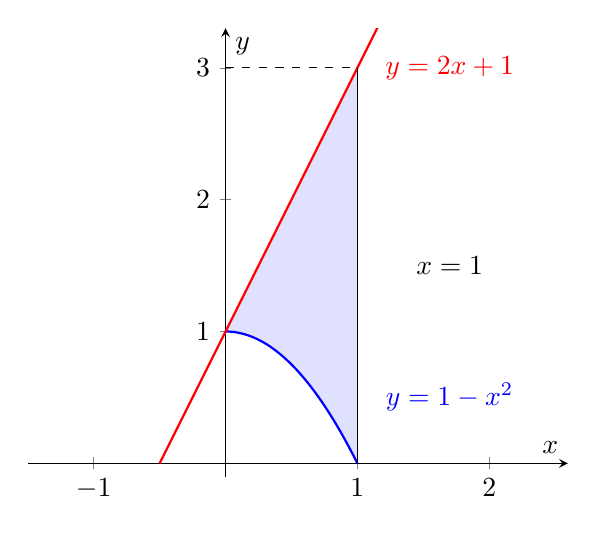
\begin{tikzpicture}
  \begin{axis}[
    axis equal,
    xlabel=$x$, ylabel=$y$,
    xmin=-0.1, xmax=1.2,
    ymin=-0.1, ymax=3.3,
    domain=0:1.2,
    samples=100,
    axis lines=middle,
    clip=true,
    scale=1,
    ]

    \addplot [
      name path=A,
      domain=0:1,
      samples=100,
      draw=none
    ] {1-x^2};

    \addplot [
      name path=B,
      domain=0:1,
      draw=none
    ] {2*x+1};

    \addplot [
      fill=blue!20,
      opacity=0.6
    ] fill between[of=A and B];

    \addplot [blue, thick, domain=0:1] {1-x^2)};
    \addplot [red, thick, domain=-0.5:1.2] {2*x+1};
    \draw (1,0)--(1,3);
    \draw[dashed] (0,3)--(1,3);
    \node[red] at (1.7,3) {$y=2x+1$};
    \node[blue] at (1.7,0.5) {$y=1-x^2$};
    \node at (1.7,1.5) {$x=1$};
  \end{axis}
\end{tikzpicture}
\end{minipage}
\begin{minipage}{0.4\textwidth}
\[\boxed{\int_0^1\int_{1-x^2}^{2x+1}f(x,y)\,dy\,dx}\]
\end{minipage}
\end{center}

\hfill

\noindent (b) Sketch the region.

\hfill

\begin{center}
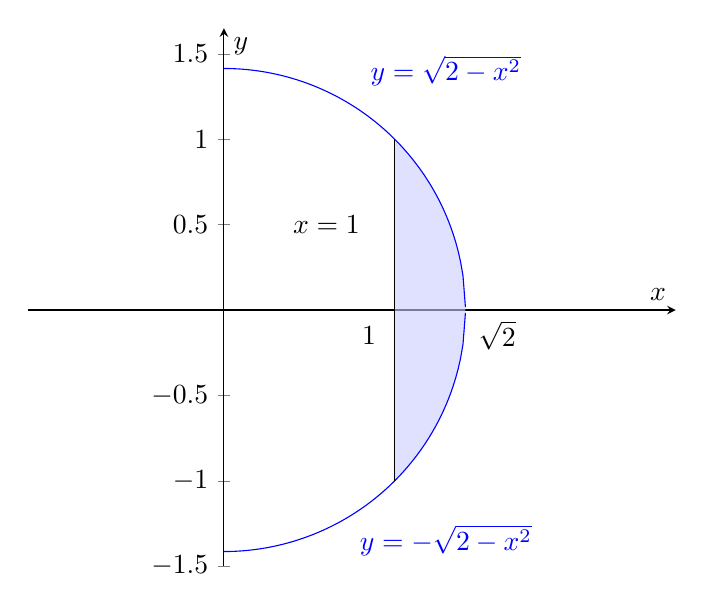
\begin{tikzpicture}
  \begin{axis}[
    axis equal,
    xlabel=$x$, ylabel=$y$,
    xmin=0, xmax=1.5,
    ymin=-1.5, ymax=1.65,
    xtick=\empty,
    domain=0:1.5,
    samples=100,
    axis lines=center,
    clip=true,
    scale=1.2,
    ]
    
    \addplot [
      domain=0:sqrt(2),
      samples=100,
      blue
    ] {sqrt(2-x^2)};
    
    \addplot [
      domain=0:sqrt(2),
      samples=100,
      blue
    ] {-sqrt(2-x^2)};

    \addplot [
      name path=A,
      domain=1:sqrt(2),
      draw=none
    ] {sqrt(2-x^2)};
    
    \addplot [
      name path=B,
      domain=1:sqrt(2),
      draw=none
    ] {-sqrt(2-x^2)};

    \addplot [
      fill=blue!20,
      opacity=0.6
    ] fill between[of=A and B];

    \draw (1,1)--(1,-1);
    \draw[dashed] (0,3)--(1,3);
    \node[red] at (1.7,3) {$y=2x+1$};
    \node[blue] at (1.3,1.4) {$y=\sqrt{2-x^2}$};
    \node[blue] at (1.3,-1.35) {$y=-\sqrt{2-x^2}$};
    \node at (0.6,0.5) {$x=1$};
    \node at (0.85,-0.15) {$1$};
    \node at (1.6,-0.15) {$\sqrt2$};
  \end{axis}
\end{tikzpicture}
\end{center}

\hfill

\[\mathrm{I}=\int_1^{\sqrt2}\int_{-\sqrt{2-x^2}}^{\sqrt{2-x^2}}\sqrt{x^2+y^2}\,dy\,dx\]

\hfill

\noindent We may switch to polar coordinates to easily evaluate the integral.

\[
\begin{array}{c}
x=r\cos\theta\\
y=r\sin\theta\\[0.2cm]
\displaystyle\theta=\tan^{-1}\frac yx\\[0.2cm]
x^2+y^2=r^2\\
dA=dy\,dx =r\,dr\,d\theta
\end{array}\quad\rightarrow\quad
\begin{array}{c}
x=\sqrt2\cos\theta,\quad y=\sqrt2\sin\theta,\quad r_{\text{upper}}=\sqrt2\\[1em]
x=1\implies r\cos\theta=1\implies r_{\text{lower}}=\sec\theta\\[1em]
\displaystyle1=\sqrt2\cos\theta\implies\cos\theta=\frac1{\sqrt2}\implies\theta=\pm\frac\pi4\\[1em]
0\leq\theta\leq \pi/2\\
\end{array}
\]

\begin{align}\mathrm{I}&=\int_{-\pi/4}^{\pi/4}\int_{\sec\theta}^{\sqrt2}r\cdot r\,dr\,d\theta=\int_{-\pi/4}^{\pi/4}\left[\frac{r^3}3\right]_{r=\sec\theta}^{r=\sqrt2}\,d\theta=\frac13\int_{-\pi/4}^{\pi/4}\left(2\sqrt2-\sec^3\theta\right) \,d\theta\nonumber\\\nonumber\\&=\int_{-\pi/4}^{\pi/4}\frac{2\sqrt2}3\,d\theta-\frac13\int_{-\pi/4}^{\pi/4}\sec^3\theta\,d\theta\end{align}

\hfill

\noindent Evaluate the left-hand side integral in $(1)$.

\[\int_{-\pi/4}^{\pi/4}\frac{2\sqrt2}3\,d\theta=\frac{2\sqrt2}3\cdot\theta\,\bigg|_{-\pi/4}^{\pi/4}=\frac{\pi\sqrt2}3\]

\hfill

\noindent Evaluate the right-hand side integral in $(1)$ with the help of integration by parts.

\begin{align*}u=\sec\theta\,&\rightarrow\,du=\sec\theta\tan\theta\,d\theta\\dv=\sec^2\theta\,d\theta\,&\rightarrow\,v=\tan\theta\end{align*}

\begin{align*}
\int\sec^3\theta\,d\theta&=\tan\theta\cdot\sec\theta-\int\tan^2\theta\sec\theta\,d\theta=\tan\theta\cdot\sec\theta-\int\frac{1-\cos^2\theta}{\cos^3\theta}\,d\theta\\\\&=\tan\theta\cdot\sec\theta-\int\sec^3\theta\,d\theta+\int\sec\theta\,d\theta
\end{align*}

\hfill

\noindent Notice that the integral of $\sec^3\theta$ with respect to $\theta$ appears on the right side of the equation. Perform some algebra and then find the result of the integral.

\begin{equation*}\int\sec^3\theta\,d\theta=\frac12\cdot\tan\theta\cdot\sec\theta+\frac12\cdot\int\sec\theta\,d\theta\end{equation*}

\hfill

\noindent The integral of $\sec\theta$ with respect to $\theta$ is as follows.

\begin{equation*}\int\sec\theta\,d\theta=\ln\left|\tan\theta+\sec\theta\right|+c_0,\quad c_0\in\mathbb{R}\end{equation*}

\hfill

\noindent Rewrite $(1)$.

\begin{align*}\mathrm{I}&=\frac{\pi\sqrt2}3-\frac13\cdot\frac12\left(\tan\theta\cdot\sec\theta+\ln\left|\tan\theta+\sec\theta\right|\right)\bigg|_{-\pi/4}^{\pi/4}\\\\&=\frac{\pi\sqrt2}3-\frac16\left[\left(1\cdot\sqrt2+\ln\left(1+\sqrt2\right)\right)-\left(-1\cdot\sqrt2+\ln\left(-1+\sqrt2\right)\right)\right]\\\\&=\boxed{\frac{(\pi-1)\sqrt2}3+\frac16\cdot\ln\left(\frac{1+\sqrt2}{-1+\sqrt2}\right)}\end{align*}

\hfill

\noindent 3. From the bounds of the integral given in cylindrical coordinates, we infer that this is the region bounded above by the sphere $x^2+y^2+z^2=4$ and bounded below by the cone $z^2=x^2+y^2$ 

\hfill

\noindent (a)

\[
\begin{array}{c}
z=z\\
x=r\cos\theta\\
y=r\sin\theta\\
r^2=x^2+y^2\\
dV=r\,dz\,dr\,d\theta=dz\,dy\,dx
\end{array}\quad\rightarrow\quad
\begin{array}{c}
z=\sqrt{4-r^2}\implies z=\sqrt{4-x^2-y^2}\\
z=r\implies z=\sqrt{x^2+y^2}\\[1em]
0\leq\theta\leq2\pi,\quad 0\leq r\leq\sqrt2\\[0.2cm]
\downarrow\\[0.2cm]
-\sqrt{2-y^2}\leq y\leq\sqrt{2-y^2},\quad -\sqrt2\leq y\leq\sqrt2
\end{array}
\]

\[\boxed{\int_{-\sqrt2}^{\sqrt2}\int_{-\sqrt{2-y^2}}^{\sqrt{2-y^2}}\int_{\sqrt{x^2+y^2}}^{\sqrt{4-x^2-y^2}}3\,dz\,dx\,dy}\]

\hfill

\noindent (b) For spherical coordinates, we have

\[
\begin{array}{c}
z=\rho\cos\phi\\
r=\rho\sin\phi\\
x^2+y^2+z^2=\rho^2\\
dV=\rho^2\sin\phi\,d\rho\,d\phi\,d\theta
\end{array}\rightarrow
\begin{array}{c}
z=\sqrt{4-r^2}\implies\rho\cos\phi=\sqrt{4-\rho^2\sin^2\phi}\implies\rho_{\text{upper}}=2\\
z=r\implies\rho\cos\phi=\rho\sin\phi\implies\rho_{\text{lower}}=0\\[1em]
\displaystyle\cos\phi=\sin\phi\implies\tan\phi=1\implies\phi_{\text{upper}}=\frac\pi4\\
\phi_{\text{lower}}=0,\quad 0\leq\theta\leq2\pi
\end{array}
\]

\[\boxed{\int_0^{2\pi}\int_{0}^{\pi/4}\int_0^23\rho^2\sin\phi\,d\rho\,d\phi\,d\theta}\]

\hfill

\noindent 4.

\hfill

\noindent (a) For $\mathbf{F}$ to be conservative, it must be the gradient of some potential function $\phi$. We may apply the component test to determine whether mixed partial derivatives are equal.

\hfill

\[
\left.
\begin{array}{l}
\displaystyle\frac{\partial\mathrm{F}_1}{\partial y}=2x\cos\left(x^2y\right)-2xy\sin\left(x^2y\right)\cdot x^2\\[1em]
\displaystyle\frac{\partial\mathrm{F}_2}{\partial x}=-2x\cos\left(x^2y\right)+x^2\sin\left(x^2y\right)\cdot 2xy
\end{array}\right\}\implies\displaystyle\frac{\partial\mathrm{F}_1}{\partial y}\neq\displaystyle\frac{\partial\mathrm{F}_2}{\partial x}
\]

\hfill

\noindent The mixed partial derivatives are not equal. Therefore, the force is not conservative.

\hfill

\noindent (b) Like what we did above, determine the mixed partial derivatives.

\[
\begin{array}{c}
\displaystyle\frac{\partial\mathrm{F}_1}{\partial y}=2y\cos\left(xy^2\right)-y^2\sin\left(xy^2\right)\cdot2xy+z^2)=\frac{\partial\mathrm{F}_2}{\partial x}\\[1em]
\displaystyle\frac{\partial\mathrm{F}_1}{\partial z}=2yz=\frac{\partial\mathrm{F}_3}{\partial x}\\[1em]
\displaystyle\frac{\partial\mathrm{F}_2}{\partial z}=2xz+\mathrm{e}^{yz}+zy\mathrm{e}^{yz}=\frac{\partial\mathrm{F}_3}{\partial y}
\end{array}
\]

\hfill

\noindent (c) Since $\mathbf{F}$ is conservative on $\mathbb{R}^3$, there exists a potential function $f$ such that $\nabla f=\mathbf{F}$.

\[\frac{\partial f}{\partial x}=y^2\cos\left(xy^2\right)+yz^2,\quad\frac{\partial f}{\partial y}=2xy\cos\left(xy^2\right)+xz^2+z\mathrm{e}^{yz},\quad\frac{\partial f}{\partial z}=2xyz+y\mathrm{e}^{yz}+2z\]

\[\int\frac{\partial f}{\partial x}\,dx=\int\left(y^2\cos\left(xy^2\right)+yz^2\right)\,dx=\sin\left(xy^2\right)+xyz^2+g(y,z)=f(x,y,z)\]

\begin{align*}\frac{\partial f}{\partial y}&=\frac{\partial}{\partial y}\left(\sin\left(xy^2\right)+xyz^2+g(y,z)\right)=2xy\cos\left(xy^2\right)+xz^2+g_y(y,z)\\\\&=2xy\cos\left(xy^2\right)+xz^2+z\mathrm{e}^{yz}\implies g_y(y,z)=z\mathrm{e}^{yz}\end{align*}

\[\int\frac{\partial f}{\partial y}\,dy=\int\left(2xy\cos\left(xy^2\right)+xz^2+z\mathrm{e}^{yz}\right)\,dy=\sin\left(xy^2\right)+xyz^2+\mathrm{e}^{yz}+h(z)=f(x,y,z)\]

\begin{align*}\frac{\partial f}{\partial z}&=\frac{\partial}{\partial z}\left(\sin\left(xy^2\right)+xyz^2+\mathrm{e}^{yz}+h(z)\right)=2xyz+y\mathrm{e}^{yz}+h_z(z)\\\\&=2xyz+y\mathrm{e}^{yz}+2z\implies h_z(z)=2z\end{align*}

\[\int\frac{\partial f}{\partial z}\,dz=\int\left(2xyz+y\mathrm{e}^{yz}+2z\right)\,dz=\sin\left(xy^2\right)+xyz^2+\mathrm{e}^{yz}+z^2+c=f(x,y,z)\]

\hfill

\noindent The potential function for $\mathbf{F}$ is

\[\boxed{f(x,y,z)=\sin\left(xy^2\right)+xyz^2+\mathrm{e}^{yz}+z^2+c,\quad c\in\mathbb{R}}\]

\hfill

\noindent 5.

\hfill

\noindent (a) We showed that $\mathbf{F}$ is conservative in $4(b)$. Using the Fundamental Theorem of Line Integrals, evaluate $f(0,1,3)-f(1,0,2)$.

\begin{align*}\int_D\mathbf{F}\cdot d\mathbf{r}&=f(0,1,3)-f(1,0,2)=\sin\left(0\right)+0+\mathrm{e}^{3}+3^2+c-\left(\sin\left(1\right)+0+\mathrm{e}^{0}+2^2+c\right)\\\\&=\boxed{\mathrm{e}^3+4}\end{align*}

\hfill

\noindent (b) The curve of intersection is a circle, which is a closed curve. Since $\mathbf{F}$ is conservative, the value of the line integral is $\boxed0$.

\hfill

\noindent 6.
\begin{center}
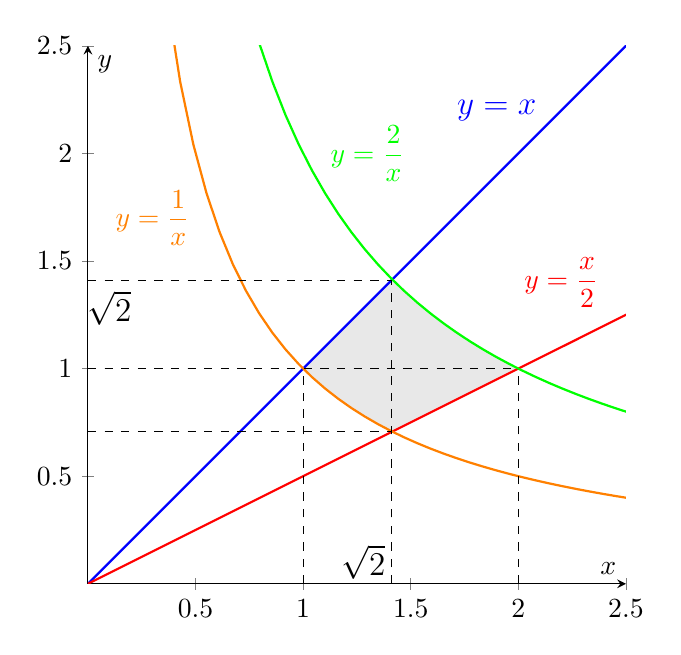
\begin{tikzpicture}
  \begin{axis}[
    axis equal image,
    xlabel=$x$, ylabel=$y$,
    xmin=0, xmax=2.5,
    ymin=0, ymax=2.5,
    domain=0:3,
    samples=50,
    axis lines=middle,
    clip=true,
    scale=1.2,
    ]

    \addplot[blue, thick] {x};
    \addplot[red, thick] {x/2};
    \addplot[green, thick] {2/x};
    \addplot[orange, thick] {1/x};
    \addplot[name path=A, draw=none, domain=1:2] {min(x,2/x)};
    \addplot[name path=B, draw=none, domain=1:2] {max(1/x,x/2)};
    \addplot[fill=gray!30, opacity=0.6] fill between[of=A and B];
    
    \draw[dashed] (1,0)--(1,1);
    \draw[dashed] (0,1)--(1,1);
    
    \draw[dashed] (1.41,0)--(1.41,1/1.41);
    \draw[dashed] (0,1/1.41)--(1.41,1/1.41);
        
    \draw[dashed] (1.41,0)--(1.41,1.41);
    \draw[dashed] (0,1.41)--(1.41,1.41);
    
    \draw[dashed] (2,0)--(2,1);
    \draw[dashed] (0,1)--(2,1);
    
    \node[blue] at (1.9,2.2) {\large $y=x$};
    \node[red] at (2.2,1.4) {$\displaystyle y=\frac x2$};
    \node[green] at (1.3,2) {$\displaystyle y=\frac2x$};
    \node[orange] at (0.3,1.7) {$\displaystyle y=\frac1x$};

    \node at (0.1,1.28) {\large $\sqrt2$};
    \node at (1.28,0.1) {\large $\sqrt2$};
  \end{axis}
\end{tikzpicture}
\end{center}

\noindent $\mathrm{F}_1$ and $\mathrm{F}_2$ have continuous partial derivatives. $C$ is a closed curve with positive orientation. We may use the tangential form of Green's Theorem to evaluate the line integral.

\begin{align*}\mathrm{I}&=\oint_C\frac{y^2}x\,dx+y\ln x\,dy=\iint_R\left(\frac{\partial\mathrm{F}_2}{\partial x}-\frac{\partial\mathrm{F}_1}{\partial y}\right)\,dA=\iint_R-\frac yx\,dA\\\\&=\int_1^{\sqrt2}\int_{1/x}^x-\frac yx\,dy\,dx+\int_{\sqrt2}^2\int_{x/2}^{2/x}-\frac yx\,dy\,dx=\int_1^{\sqrt2}-\frac{y^2}{2x}\bigg|_{y=1/x}^{y=x}\,dx+\int_{\sqrt2}^2-\frac{y^2}{2x}\bigg|_{y=x/2}^{y=2/x}\,dx\\\\&=\int_1^{\sqrt2}\left(-\frac x2+\frac{1}{2x^3}\right)\,dx+\int_{\sqrt2}^2\left(-\frac2{x^3}+\frac x8\right)\,dx=\left[-\frac{x^2}4-\frac1{4x^2}\right]_1^{\sqrt2}+\left[\frac1{x^2}+\frac{x^2}{16}\right]_{\sqrt2}^2\\\\&=\left[-\frac12-\frac18-\left(-\frac14-\frac14\right)\right]+\left[\frac14+\frac14-\left(\frac12+\frac18\right)\right]=\boxed{-\frac14}\end{align*}

\end{document}